\chapter{Versuchsplan und Durchführung}\label{ch:versuch}

% Versuchsplan
\paragraph{Der Versuchsplan (VP)} wird in der Software MiniTab \cite{minitab2026homepage} erstellt und analysiert.
Im VP sind drei Replikationen vorgesehen.
Jede Replikation wird in einem Block erfasst.
Damit werden die Streuung durch Störgrößen aus der Umwelt (Luftfeuchtigkeit, Raumtemperatur und Kühlschranktemperatur) minimiert.
Zusätzlich werden zwei Zentralpunkt pro Block vorgesehen.
Diese sollen eine spätere Prüfung auf Nichtlinearität des Modells ermöglichen.

Um schwankende Ofentemperaturen während des Backvorgangs zu vereinheitlichen, werden die Teige aller Faktorstufenkombinationen (FSK) gleichzeitig gebacken.
Damit fällt die Störgröße Blechposition mehr ins Gewicht.
Deshalb werden die Positionen in der ersten Replikation randomisiert.
Die Blechpositionen werden wie in Abbildung \ref{fig:positionen_rot} durchnummeriert.
Zudem bilden die Positionen drei Reihen (vorne, Mitte, hinten).
In der ersten Replikation ist die zufällige Durchlaufnummer gleichzeitig die Blechposition.
Für die weiteren Replikationen werden die Positionen für eine FSK systematisch rotiert.
Über die Position werden die Durchlaufnummern für die zweite und dritte Replikation definiert.
Die Rotationen sind durch rote Pfeile in der Abbildung \ref{fig:positionen_rot} dargestellt.
Mit der Rotation wird sichergestellt, dass jede FSK einmal in jeder Reihe war.
Einzig die Position 4 wird dabei nicht mitrotiert.
Auf ihr liegt immer eine FKS für den Zentralpunkt, der so unter konstanten Randbedingungen liegt.
Der entstandene Versuchsplan mit Durchlaufsnumern ist im Anhang \ref{ch:appendix_versuch} zu finden.

\begin{figure}
    \centering
    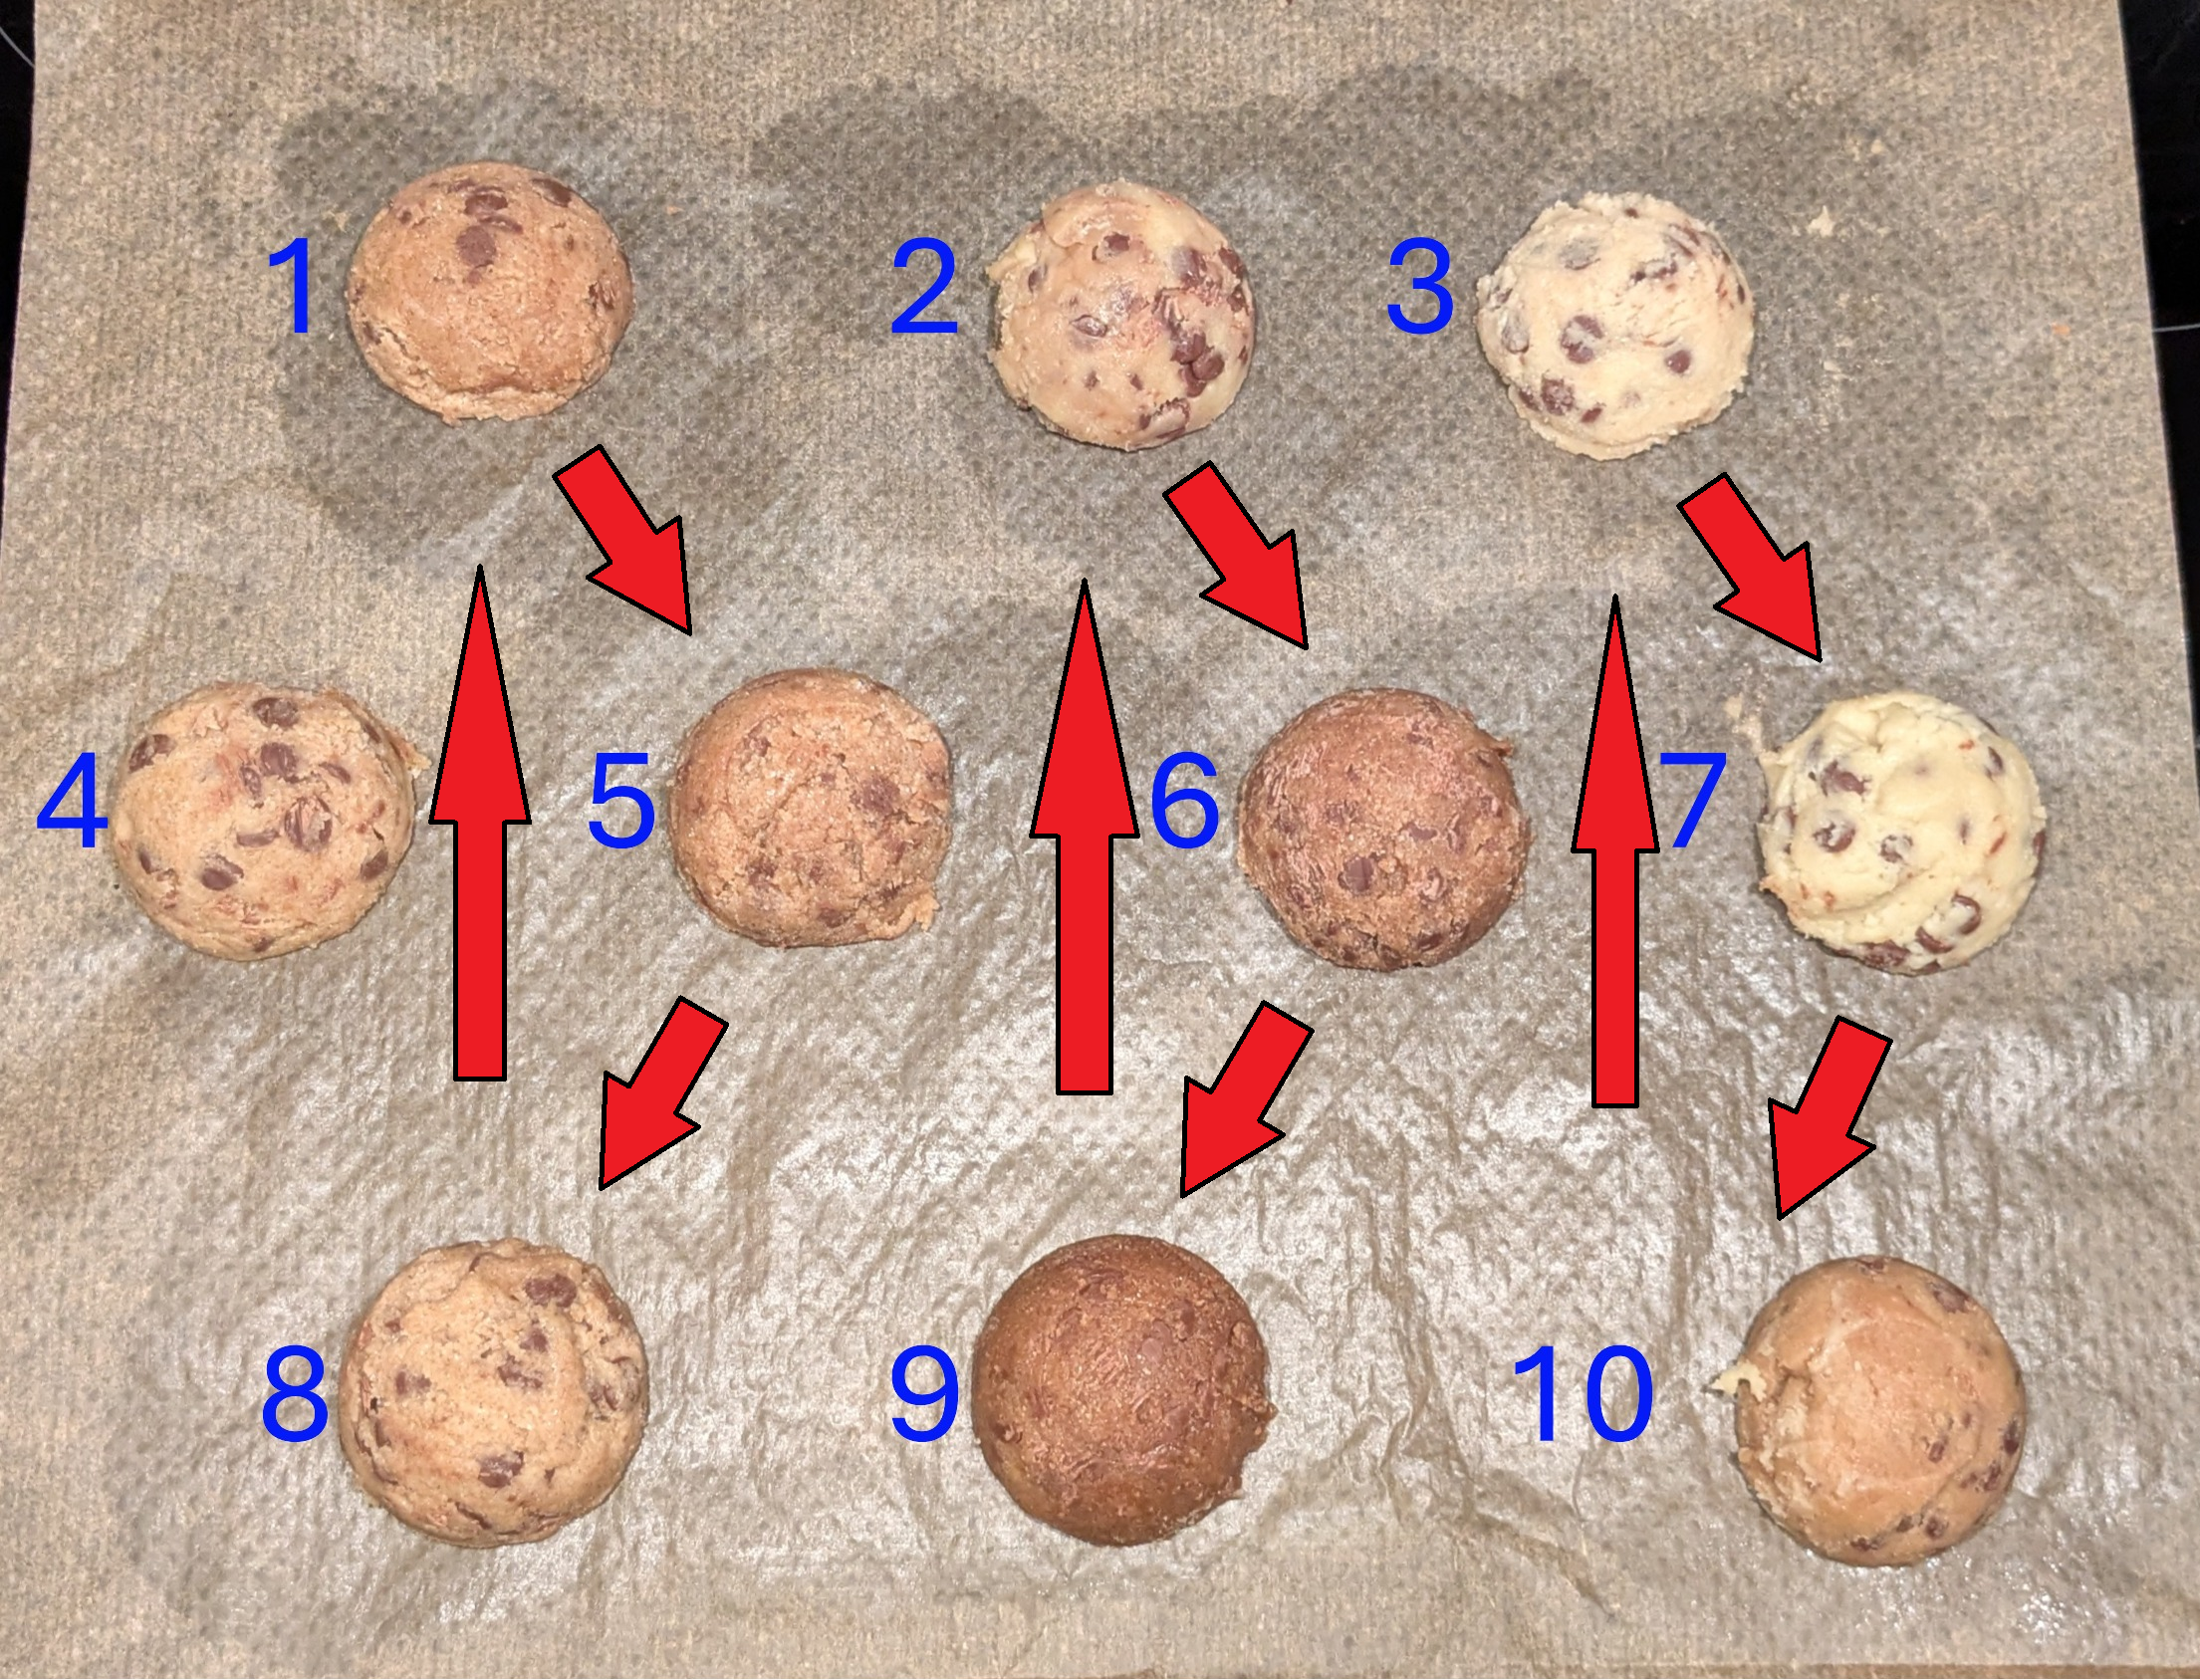
\includegraphics[width=0.7\linewidth]{figures/positionen_rot.png}
    \caption{Positionen auf dem Backblech in blau und die Rotation pro Replikation in rot.}
    \label{fig:positionen_rot}
\end{figure}

% Ablauf
\paragraph{Der Ablauf} einer Replikation wird in zwei Teilprozesse unterteilt (siehe Abbildung \ref{fig:prozess}).
Der Erste ist die Zubereitung der Teige für alle neun FSK, der Zweite das Backen und Messen der Cookies.
Dieser Ablauf wird für das Experiment drei mal durchgeführt.

\begin{figure}
    \centering
    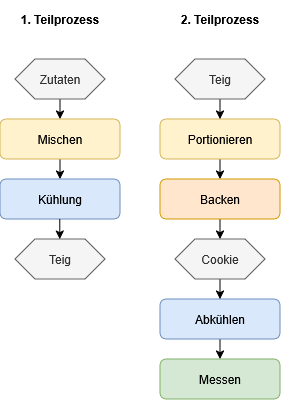
\includegraphics[width=0.4\linewidth]{figures/prozess.png}
    \caption{Prozess der Cookie-Herstellung mit zwei Teilprozessen. Links die Zubereitung des Teigs, rechts der Back- und Messvorgang.}
    \label{fig:prozess}
\end{figure}

Am Anfang einer Replikation werden alle Zutaten bereitgestellt.
Die Zutaten werden entsprechend der Prozessschritte in der Tabelle \ref{table:zubereitung_zugaben} zum Teig gegeben.
Diese Tabelle enthält auch die Temperaturen der Zutaten und das Messmittel um die Menge zu bestimmen.
Die Tabelle \ref{table:zubereitung_prozess} zeigt die Prozessschritte des Mischens.
Beide Tabellen zusammen haben eine fortlaufende Nummerierung der Prozessschritte.
Nach der Zubereitung wird der Teig in einen luftdichten Vorratsbehälter in den Kühlschrank gestellt.
Anschließend wird der Mischtopf gereinigt und getrocknet.
Dann wird mit dem Teig für die nächste FSK mit den gleichen Prozessschritten fortgefahren.
Zum Schluss des ersten Teilprozesses befinden sich neun Teige im Kühlschrank.
Dort ruhen sie für 22\,Stunden.

Am Folgetag wird zunächst der Ofen auf 175\,°C Umluft samt Backblech vorgeheizt.
Nach der Ruhezeit wird für jede FSK ein Teigrohling mit einem Eisportionierer (EP) geformt.
Der Teig wird dabei bündig zur Kante des EP abgezogen.
Anschließend wird der Teig, abzüglich des EP, gewogen.
Der Teigrohling wird auf einem Backpapier an der Blechposition entsprechend der Durchlaufnummer positioniert.
In der zweiten Replikation wird von der Durchlaufnummer zehn,
und in der dritten Replikation 20 von der Durchlaufnummer abgezogen, um auf die Position zu kommen.
Sind alle Teigrohlinge positioniert wird das Backblech aus dem Ofen entnommen und das Backpapier auf das Blech gezogen.
Das Blech wird im Ofen auf die mittlere Schiene geschoben.
Nach 11\,Minuten Backzeit wird das Blech entnommen und das Backpapier samt Cookies zum Abkühlen auf ein Gitter gezogen.
Nach 30\,Minuten Abkühlzeit werden die Cookies mit dem Messchieber vermessen.

\begin{table}
\centering
\caption{Prozessschritte der Zutatenzugaben für die Teigzubereitung}
\label{table:zubereitung_zugaben}
\begin{tabular}{|l|l|l|l|l|}
\hline
Schritt & Zutat               & Menge    & Temperatur  & Messmittel \\
\hline
1       & Butter              & nach VP     & Raum        & Küchenwaage \\
2       & Zucker              & nach VP     & Raum        & Küchenwaage \\
\hline
4       & Eier                & 2 (Größe M) & Kühlschrank & -- \\
\hline
6       & Mehl                & 280\,g      & Raum        & Küchenwaage \\
7       & Natron              & 3\,g        & Raum        & Feinwaage \\
8       & Salz                & 2\,g        & Raum        & Feinwaage \\
\hline
10      & Schokotropfen       & 100\,g      & Raum        & Küchenwaage \\
\hline
\end{tabular}
\end{table}

\begin{table}
\centering
\caption{Prozessschritte bei der Teigzubereitung}
\label{table:zubereitung_prozess}
\begin{tabular}{|l|l|l|l|l|}
\hline
Schritt & Operation & Dauer & Stufe & Gerät \\
\hline
3       & Mischen   & 40\,s & 4     & TM6 \\
5       & Mischen   & 15\,s & 4     & TM6 \\
9       & Mischen   & 20\,s & 4     & TM6 \\
11      & Mischen   & 20\,s & 3     & TM6 \\
\hline
\end{tabular}
\end{table}

% Aufwandabschätzung
\paragraph{Die Aufwandabschätzung} für das Experiment ergibt folgendes.
Die Zubereitung eines Teigs dauert circa 5\,Minuten, für neun FSK also 45\,Minuten.
Zusätzlich muss der Mischtopf neun mal gereinigt und getrocknet werden.
Das sind zusätzliche 45 Minuten, also 1,5\,Stunden für den ersten Teilprozess pro Replikation.
Während der Pause fällt kein Aufwand an.
Nur ein Teil der Kühlschrankkapazität wird für die Zeit gefordert.
Der zweite Teilprozess beinhaltet das Portionieren des Teigs zu Cookies.
Je Cookie-Portionierung wird mit anschließender Reinigung des Protionierers 1\,Minute geschätzt.
Dazu kommt das Backen im Ofen (11\,Minuten) mit anschließenden Abkühlen (30\,Minuten).
Für das Messen und übertragen der Werte werden 19\,Minuten eingeplant.
Pro Replikation werden 1\,Stunde für den zweiten Teilprozess und 2,5\,Stunden im Gesamten benötigt.
Der Aufwand für das Gesamte Experiment liegt damit bei 7,5\,Stunden verteilt auf 6 Tage.

% Vorversuch
\paragraph{Der Vorversuch} brachte wichtige Erkenntnisse. 
So wurden im Vorversuch Stückchen einer weißen Tafel Schokolade und Cranberries für die Cookies verwendet.
Die unterschiedlich großen Schokoladenstückchen und Cranberries führten zu starken variierenden Cookie-Formen.
Die Cookies aus dem Vorversuch sind in Abbildung \ref{fig:vorversuch} im Anhang \ref{ch:appendix_vorversuch} zu sehen.
Im Experiment werden deshalb Schokoladentropfen (SchokoTro) verwendet.
Diese sind maschinell gefertig und deutlich konsistenter in ihrer Größe.

Der Vorversuch nutzte zwei Extreme des Faktorraums.
Einen Teig mit 0\,\% Vollkornmehl, minimaler Zucker- und Buttermenge und ein Teig mit maximaler Zucker- und Buttermenge mit 0\,\% Vollkornmehl.
Dabei zeigten sich deutliche Unterschiede im Durchmesser und der Höhe der Cookies.
Es zeigte sich zudem, dass der Messzeitpunkt für den Durchmesser nach dem Backen nicht relevant ist.
Bei der Höhe sind 30 Minuten nach der Entnahme aus dem Ofen keine Änderungen messbar.

% ToDo
%Bestätigungsversuche ?! - Teig irgendwo im Raum, durch Formel berechnet